% Created 2019-03-08 Fri 15:09
% Intended LaTeX compiler: pdflatex
\documentclass[11pt]{article}
\usepackage[utf8]{inputenc}
\usepackage[T1]{fontenc}
\usepackage{graphicx}
\usepackage{grffile}
\usepackage{longtable}
\usepackage{wrapfig}
\usepackage{rotating}
\usepackage[normalem]{ulem}
\usepackage{amsmath}
\usepackage{textcomp}
\usepackage{amssymb}
\usepackage{capt-of}
\usepackage{hyperref}
\usepackage{minted}
\author{Heitor Lourenço Werneck \\{\href{mailto:heitorwerneck@hotmail.com}{heitorwerneck@hotmail.com}}}
\usepackage[portuguese]{babel}
\usepackage{amsmath}
\usepackage[binary-units=true]{siunitx}
\usepackage[top=0.5cm,bottom=2cm,left=2cm,right=2cm]{geometry}
\usemintedstyle{rainbow_dash}
\usepackage{mdframed}
\date{\today}
\title{Algoritmos e Estrutura de Dados II (2018-2)\\\medskip
\large Trabalho Prático 2}
\hypersetup{
 pdfauthor={Heitor Lourenço Werneck},
 pdftitle={Algoritmos e Estrutura de Dados II (2018-2)},
 pdfkeywords={},
 pdfsubject={},
 pdfcreator={Emacs 26.1 (Org mode 9.1.9)}, 
 pdflang={Portuguese}}
\begin{document}

\maketitle
\tableofcontents

\definecolor{bg}{rgb}{0.95,0.95,0.95}
\BeforeBeginEnvironment{minted}{\begin{mdframed}[backgroundcolor=bg]}
\AfterEndEnvironment{minted}{\end{mdframed}}
\newpage
\section{Introdução}
\label{sec:org57f5db9}

O trabalho apresentado nesse documento consiste na avaliação do método de ordenação quicksort (recursivo) considerando as seguintes entradas:
\begin{itemize}
\item Os elementos a serem ordenados são inteiros armazenados em um vetor de tamanho N.
\item Os  elementos  a  serem  ordenados  são  inteiros  armazenados  em  uma  lista  duplamente  encadeada  com N elementos.
\item Os  elementos  a  serem  ordenados  são  registros  armazenados  em  um  vetor  de  tamanho N.
\end{itemize}
\paragraph{Cada registro contém:}
\begin{itemize}
\item Um inteiro, a chave para ordenação.
\item Dez cadeias de caracteres (strings), cada uma como 200 caracteres.
\item 1 booleano.
\item 4 números reais.
\end{itemize}

\paragraph{As entradas para o programa são:}
\begin{enumerate}
\item semente.
\item arquivo de entrada.
\item arquivo de saída.
\end{enumerate}
No arquivo de entrada a primeira linha contém o número de valores que se seguem e os próximos valores são o tamanho das sequencias(N) a serem geradas.

Também foi necessário implementar funções para criação dos conjuntos de elementos aleatórios.

\subsection{Funcionamento do algoritmo (Visão geral)}
\label{sec:org71febc1}
Com o arquivo de entrada, a primeira coisa é ler a primeira linha para saber quantos valores de tamanho de vetor(N's) se seguem. 

Apos isso, o programa prossegue lendo os N's, e a cada leitura de um N o programa irá entrar em um laço de repetição que ira ser repetido 5 vezes (definido na especificação do trabalho), e dentro desse laço ocorre a atribuição da semente (a semente se diferencia para cada um das 5 repetições para gerar valores diferentes) a geração de valores randômicos de cada tipo de lista é feita assim como a ordenação, as estatísticas da ordenação são guardadas. No final das 5 repetições é feito uma media de cada algoritmo para cada tipo de lista.

Já no final do algoritmo todos os N's terão suas estatísticas no arquivo de saída.

\newpage
\section{Implementação}
\label{sec:org217c4b1}
\subsection{Estruturas de dados}
\label{sec:orgd4efad6}
As estruturas utilizadas foram:

\begin{enumerate}
\item Vetor de inteiro (\mintinline{c}{int *vint = malloc(sizeof(int)*N)});

\item Lista duplamente encadeada de inteiros

\begin{minted}[]{c}
struct TLista
{
  struct TCelula* inicio;
  int tamanho;
  struct TCelula* fim;
};

struct TCelula
{
  struct TCelula* ant;
  int valor;
  struct TCelula* prox;
};

typedef struct TLista lista;
typedef struct TCelula celula;
\end{minted}

\item vetor de struct

\begin{minted}[]{c}
#define numstr 10
#define strsize 200
#define realn 4
#define booltotaln 2
typedef char bool;
typedef struct elem{
  int ch;//Chave para ordenação
  char str[numstr][strsize];//numstr strings, cada uma com strsize caracters
  bool b; // booleano
  float r[realn];//numeros reais
}elem;
\end{minted}

\item Informações sobre algoritmo (algoinfo)
Essa estrutura de dados foi necessária para guardar informações do algoritmo quicksort a ser executado para depois ser possível guardar as estatísticas, essa estrutura guarda:
\begin{itemize}
\item Numero de ativações
\item Copias ou trocas
\item Comparações
\item Tempo de usuário
\item Tempo do sistema
\item Tempo total
\end{itemize}
\end{enumerate}

\subsection{Gerador aleatório}
\label{sec:orgfd43170}
O gerador aleatório se diferencia para cada tipo de dado:

\begin{description}
\item[{int}] Para gerar um inteiro aleatório foi feito uma logica simples \mintinline{c}{rand()%(size*randn)}, isso basta para não ter grande variabilidade de valores para pequenos valores de N e se for maior terá maior variabilidade.
\item[{string}] Para a geração de string é necessário um conjunto de caracteres permitidos na geração aleatória, o conjunto de caracteres utilizado foi o abaixo:
\begin{minted}[]{c}
const char charset[] =
  "0123456789abcdefghijklmnopqrstuvwxyzABCDEFGHIJKLMNOPQRSTUVWXYZ";
\end{minted}
Basta fazer o modulo do tamanho do conjunto de caracteres.
\begin{minted}[]{c}
charset[rand()%sizeof(charset)];
\end{minted}

\item[{bool}] a geração do booleano basta utilizar o modulo de 2 para obter-se valores 0 ou 1.
\begin{minted}[]{c}
rand()%booltotaln;
\end{minted}
\item[{float}] para gerar um float basta dividir o rand()(um valor inteiro) por um valor float, a lógica seguinte faz com que seja possível um numero float aleatório.
\begin{minted}[]{c}
(float)rand()/(float)(RAND_MAX/(size*randn));
\end{minted}

As seguintes funções são dos geradores para cada tipo de estrutura de dados.
\end{description}
\begin{minted}[]{c}
void vint_random(int *vint, size_t size);
void lint_random(lista *lint, size_t max);
void struct_random(elem *vstruct, size_t size);
\end{minted}

\subsection{Semente}
\label{sec:org47d06d6}
Para a utilização da semente só foi necessário uma logica que durante as 5 repetições tivesse uma diferenciação na semente, como especificado.
\begin{minted}[]{c}
for(int nsed=0;nsed<repeat;nsed++){
  srand(atoi(argv[seed])+nsed*randn);
  ...
    }
\end{minted}

\subsection{Contador de tempo}
\label{sec:org32f7e7a}
Para contar o tempo que cada quicksort utiliza foi necessário a criação da seguinte função:

\mintinline{c}{void timeusage(struct rusage *resources,char start,algoinfo *ai);}.
\begin{itemize}
\item a estrutura rusage é a estrutura que vai guardar o tempo na forma "original".
\item o carácter start é uma variável utilizada para saber se é para começar a contar ou parar, se start for verdadeiro então começara a contar o tempo, se for falso ira parar de contar.
\item a estrutura algoinfo irá guardar o tempo total, de usuário e do sistema.
\end{itemize}
\subsection{Quicksort}
\label{sec:org8be48cf}
Como há 3 estruturas de dados diferentes será necessário 3 algoritmos de quicksort diferentes.
\subsubsection{Vetor de inteiro}
\label{sec:org587fcad}
\begin{minted}[]{c}
int particiona_int(int vetor[], int inicio, int fim,algoinfo* ai);
void quick_int(int vetor[], int inicio, int fim, algoinfo* ai);
\end{minted}
Aqui foi feito o quicksort padrão que normalmente é feito para vetor de inteiros. A função particiona\_int reorganiza o vetor em torno de um pivô escolhido, que no caso dessa implementação o pivô é o primeiro numero, e apos isso vai dividindo e reorganizando o vetor ate chegar em elementos individuais e no final o resultado será o vetor organizado.

Na reorganização é utilizado duas variáveis para movimentação pelo vetor, que são as variáveis \textbf{esq} e \textbf{dir} e a variável \textbf{esq} inicia com o índice inicial e a variável \textbf{dir} inicia com o índice final, um laço é repetido enquanto a variável \textbf{esq} for menor que a \textbf{dir}. 

Dentro desse laço existe um laço para movimentação da variável \textbf{esq} que enquanto o valor na posição \textbf{esq} do vetor for menor ou igual ao pivô e enquanto a \textbf{esq} for menor que \textbf{fim} o laço irá movimentar uma posição positivamente na variável \textbf{esq} ou seja aumentar 1 na \textbf{esq}.

Dentro desse laço também existe um laço para movimentação da variável \textbf{dir} que enquanto o valor na posição \textbf{dir} do vetor for maior que o pivô o laço irá movimentar uma posição negativamente na variável \textbf{dir} ou seja diminuir 1 em \textbf{dir}.

Depois se o \textbf{esq} ainda for menor que \textbf{dir} então o valor nesses índices terão valores trocados.

Então quando acaba todo o while e \textbf{esq} é maior ou igual a \textbf{dir} então a posição inicial recebe o valor no índice \textbf{dir} e o valor no índice \textbf{dir} recebe o valor do pivô. E no final o retorno será \textbf{dir} que é o índice que irá dividir o vetor.

Durante todo esse processo as informações do algoritmo são armazenadas na variável \textbf{ai}.
\begin{minted}[]{c}
int particiona_int(int vetor[], int inicio, int fim,algoinfo* ai)
{
  int esq, dir;
  int pivo, aux;
  esq = inicio;
  dir = fim;
  pivo = vetor[inicio];
  while(esq<dir)
  {
    while(vetor[esq] <= pivo && esq<fim){   // vetor[esq] <= pivo
      esq++;
      ai->comparacoes++;
    }

    while(pivo < vetor[dir]){    //  vetor[dir] > pivo
      dir--;
      ai->comparacoes++;
    }

    if(esq < dir)
    {
      aux = vetor[esq];          // troca vetor[esq] com vetor[dir]
      vetor[esq] = vetor[dir];
      vetor[dir] = aux;
      ai->troca++;
    }

    ai->comparacoes+=comparasionnumber;
  }

  ai->comparacoes++;
  vetor[inicio] = vetor[dir];
  vetor[dir] = pivo;
  return dir;                   //retorna dir, que é o índice que vai dividir o vetor
}


void quick_int(int vetor[], int inicio, int fim, algoinfo* ai)
{
  ai->ativacoes++;
  int pivo;
  if(inicio < fim)
  {
    pivo = particiona_int(vetor,inicio,fim,ai); // encontra um pivo que "divide" o vetor em dois
    quick_int(vetor, inicio, pivo-1, ai); // realiza a partição para a parte da esquerda
    quick_int(vetor, pivo+1, fim, ai);  // e realiza a partição para a parte de direita
  }
}
\end{minted}
\subsubsection{Lista duplamente encadeada de inteiro}
\label{sec:orgf7e7a89}
\begin{minted}[]{c}
celula* particiona_int_l(celula* inicio, celula* fim,algoinfo* ai);
void quick_int_l(celula* inicio,celula* fim,algoinfo* ai);
\end{minted}

O quicksort para lista duplamente encadeada encontra algumas pequenas diferenças como nos tipos de dados utilizados para se fazer a ordenação. A função particiona\_int\_l reorganiza a lista em torno de um pivô escolhido, que no caso dessa implementação o pivô é o primeiro numero, e apos isso vai dividindo e reorganizando o vetor ate chegar em elementos individuais e no final o resultado será o vetor organizado.

Para a equivalência de \textbf{esq<dir} como no quicksort para vetor de inteiros foi feito um macro que irá resolver o problema.

\begin{minted}[]{c}
#define LLTR(left, right)  (right != NULL && left != right && left != right->prox)

\end{minted}

Esse macro irá receber dois ponteiros de celula e irá dizer se o ponteiro da esquerda é menor que o segundo em relação a posição na lista.

Na reorganização é utilizado duas variáveis para movimentação pela lista, que são as variáveis \textbf{esq} e \textbf{dir} e a variável \textbf{esq} inicia apontando para a celula inicial e a variável \textbf{dir} inicia apontando para a celula final, um laço é repetido enquanto a variável \textbf{esq} for menor que a *dir*(\texttt{LLTR(esq,dir)}). 

Dentro desse laço existe um laço para movimentação da variável \textbf{esq} que enquanto o valor na \textbf{esq} for menor ou igual ao pivô e enquanto a \textbf{esq} for menor que \textbf{fim} a \textbf{esq} irá para a próxima celula.

Dentro desse laço também existe um laço para movimentação da variável \textbf{dir} que enquanto o valor de \textbf{dir} for maior que o pivô o laço irá para a celula anterior a \textbf{dir}.

Depois se o \textbf{esq} ainda for menor que \textbf{dir} então o valor nessas celulas serão trocados.

Então quando acaba todo o while e \textbf{esq} é maior ou igual a \textbf{dir} então a celula \textbf{inicio} recebe o valor de \textbf{dir} e o valor de \textbf{dir} recebe o valor do pivô. E no final o retorno será \textbf{dir} que é a celula que irá dividir a lista.

Durante todo esse processo as informações do algoritmo são armazenadas na variável \textbf{ai}.

\begin{minted}[]{c}

celula* particiona_int_l(celula* inicio, celula* fim,algoinfo* ai){
  int pivo = inicio->valor,aux;
  celula* dir = fim,*esq = inicio;
  while(LLTR(esq,dir)){
    while(esq->valor <= pivo && LLTR(esq,fim)){
      esq=esq->prox;
      ai->comparacoes++;
    }
    while(pivo < dir->valor){
      dir=dir->ant;
      ai->comparacoes++;
    }
    if(LLTR(esq,dir))
    {
      aux = dir->valor;
      dir->valor = esq->valor;
      esq->valor = aux;
      ai->troca++;
    }
    ai->comparacoes+=comparasionnumber;
  }
  ai->comparacoes++;
  inicio->valor = dir->valor;
  dir->valor = pivo;
  return dir;
}

void quick_int_l(celula* inicio,celula* fim,algoinfo* ai){
  ai->ativacoes++;
  if (LLTR(inicio,fim)){
    celula* pivo =  particiona_int_l(inicio,fim,ai);
    quick_int_l(inicio, pivo->ant,ai);
    quick_int_l(pivo->prox, fim,ai);
  }
}
\end{minted}
\subsubsection{Vetor de registro}
\label{sec:org1d39db1}
\begin{minted}[]{c}
int particiona_struct(elem* rgs, int inicio, int fim,algoinfo* ai);
void quick_struct(elem* rgs, int inicio, int fim, algoinfo* ai);
\end{minted}

Este quicksort é bem parecido com o padrão que normalmente é feito para vetor de inteiros. A função particiona\_struct reorganiza o vetor em torno de um pivô escolhido, que no caso dessa implementação o pivô é a chave do primeiro elemento do vetor, e apos isso vai dividindo e reorganizando o vetor ate chegar em elementos individuais e no final o resultado será o vetor organizado.

Para fazer o quicksort em uma struct basta selecionar um de seus elementos e utilizá-lo como um valor de referencia para ordenação. Nesse caso o valor utilizado foi o campo \textbf{ch} que é um inteiro.

Quase tudo ira ser como na ordenação de vetor de inteiros. Agora para acessar um índice em certa posição basta também utilizar o acesso ao elemento \textbf{ch} que será o valor de referencia.

Na troca de valores o registro deverá ser trocado completamente e necessitara de um auxiliar do tipo \textbf{elem} para a troca ser efetuada. Diferente da troca das outras estruturas que só necessitavam de trocar um inteiro.

Durante todo esse processo as informações do algoritmo são armazenadas na variável \textbf{ai}.

\begin{minted}[]{c}
int particiona_struct(elem* rgs, int inicio, int fim,algoinfo* ai)
{
  int esq, dir;
  elem pivo,aux;
  esq = inicio;
  dir = fim;
  pivo = rgs[inicio];
  while(esq<dir)
  {
    while(rgs[esq].ch <= pivo.ch && esq<fim){
      esq++;
      ai->comparacoes++;
    }

    while(pivo.ch < rgs[dir].ch){
      dir--;
      ai->comparacoes++;
    }

    if(esq < dir)
    {
      aux = rgs[esq]; 
      rgs[esq] = rgs[dir];
      rgs[dir] = aux;
      ai->troca++;
    }

    ai->comparacoes+=comparasionnumber;
  }

  ai->comparacoes++;
  rgs[inicio] = rgs[dir];
  rgs[dir] = pivo;
  return dir;                   //retorna dir, que é o índice que vai dividir o rgs
}

void quick_struct(elem* rgs, int inicio, int fim,algoinfo* ai)
{
  ai->ativacoes++;
  int pivo;
  if(inicio < fim)
  {
    pivo = particiona_struct(rgs,inicio,fim,ai); // encontra um pivo que "divide" o vetor em dois
    quick_struct(rgs, inicio, pivo-1, ai); // realiza a partição para a parte da esquerda
    quick_struct(rgs, pivo+1, fim, ai);  // e realiza a partição para a parte de direita
  }
}
\end{minted}
\subsection{Saida dos resultados}
\label{sec:orge112561}
A função a seguir é responsável por imprimir no arquivo de saída os dados de cada algoritmo. Ela recebe uma estrutura do tipo algoinfo que contem informações do algoritmo e ira imprimir todas informações.
\begin{minted}[]{c}
void printalgoinfo(const algoinfo *ai,FILE* f);
\end{minted}

\newpage
\section{Resultados e Discussões}
\label{sec:org1a50b92}
\begin{table}[htbp]
\centering
\begin{tabular}{|c|}
\hline
N\\
\hline
1000\\
5000\\
10000\\
50000\\
100000\\
500000\\
1000000\\
\hline
\end{tabular}
\caption{Entrada teste}

\end{table}


\captionof{table}{Saida, tempo total em segundos de cada algoritmo em media.} 
  \label{table:table_tm}
  \begin{tabular}{| c | c | c | c | c | c | c | c |}
  \hline
  & \multicolumn{7}{|c|}{N} \\\hline
  & 1000 & 5000 & 10000 & 50000 & 100000 & 500000 & 1000000 \\\hline
  Vetor de inteiro& 0.00025 & 0.00124 & 0.00249 & 0.01464 & 0.03074& 0.17130 & 0.35664 \\\hline
  Lista duplamente encadeada&0.00026 &0.00130 & 0.00268 & 0.01535 & 0.03294 & 0.18048 & 0.37783 \\ \hline
  Vetor de registro& 0.00157 & 0.01039 & 0.02445& 0.16934 & 0.36143 & 1.93895 & 4.07320 \\ \hline
  \end{tabular}

\subsubsection{Vetor de registro}
\label{sec:org9075efa}


\begin{center}
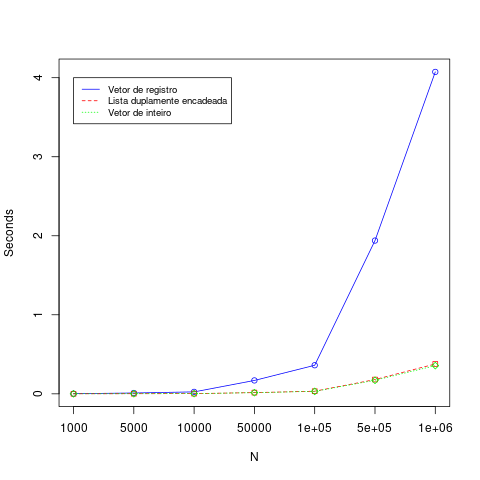
\includegraphics[width=.9\linewidth]{lists_t.png}
\end{center}

É possível ver pelo gráfico que o comportamento da lista duplamente encadeada e bastante similar ao vetor de inteiros, porém o vetor de registros tem um comportamento bastante diferente pois seu tempo de ordenação cresce de maneira descomunal.

É possível entender o porque dessa velocidade através da leitura do tamanho do registro.
Fazendo o calculo: 

\begin{equation}
\begin{aligned}
Seja: \\
sizeof(int) = 4\; bytes\\
sizeof(char) = sizeof(bool) = 1\; bytes\\
sizeof(float) = 4\; bytes\\
sizeof(elem) = sizeof(int)+sizeof(char)*10*200+sizeof(bool)+sizeof(float)*4\\
\therefore sizeof(elem) = 2021\; bytes
\end{aligned}
\end{equation}
O resultado é que o registro utiliza 2021 bytes, logo é possível entender que o custo de troca/copia de dados dessa estrutura é bastante custoso, logo isso é um dos fatores que tornam esse algoritmo mais lento pois a cada troca ele custa muito processamento. A diferença de tamanho do registro a ser trocado para as outras estruturas é significativamente maior, pois nas outras estruturas a troca é feita com variáveis inteiras que tem tamanho de 4 bytes.

O registro é 505.25 vezes maior que um inteiro (\(2021/4 = 505.25 bytes\)). Isso fala bastante sobre o custo de troca.

Será feito outro calculo de quanto de memoria é utilizado para guardar 1000000 registros(pior caso de entrada do arquivo utilizado nesse documento).

\begin{equation}
\begin{aligned}
N = 1000000\\
sizeof(elem) = 2021\; bytes\\
sizeof(elem)*N = 2021000000 \SI{0}{\byte}\\
\therefore  sizeof(elem)*N = 1927.3757 \SI{0}{\mebi\byte}
\end{aligned}
\end{equation}

É possível ver que o vetor de registro custa muita memoria com \(N = 1000000\), isso também pode atrapalhar o desempenho visto que o processador fica um tempo ocioso esperando os dados chegarem da memoria, isso é também conhecido como gargalo de Von Neumann.

\subsubsection{Vetor de inteiros e lista duplamente encadeada}
\label{sec:org93ea938}


Como na analise anterior o vetor de registro apresenta uma grande disparidade de performance com as duas outras estruturas a analise delas serão feitas nessa subseção para a melhor analise das duas estruturas.

\begin{center}
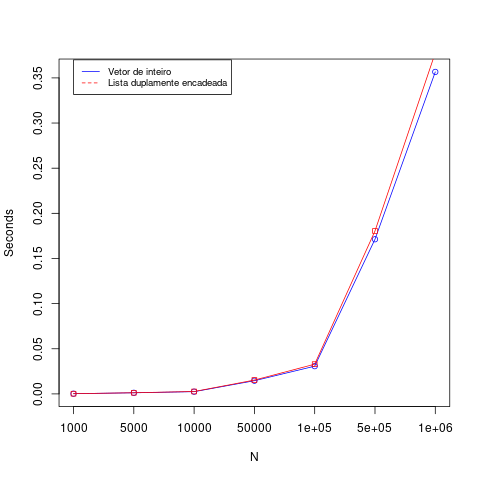
\includegraphics[width=.9\linewidth]{lint_vint_t.png}
\end{center}

Com esse gráfico um pouco mais próximo é possível observar que a lista duplamente encadeada (lint) mesmo que seja bastante próxima em performance da lista de inteiros (vint) ainda é mais lenta.

Como o \emph{vint} é uma estrutura simples sua performance é extremamente alta. É possível ver na tabela de media de tempo (\ref{table:table_tm}) no pior caso (\(N=1000000\)) a diferença de tempo de execução das duas estruturas é \(\Delta T = T_{lint}-T_{vint}=0.37783-0.35664= 0.02119s\), ou seja, 21.19\SI{}{\milli\second}. 

Sendo no pior caso a ordenação de \emph{vint} 21.19\SI{}{\milli\second} mais rápida que a ordenação em \emph{lint/(mais rápida também para todos outros N's), mesmo que o /vint} seja mais rápido por alguns milissegundos esse tempo em um processo critico pode conferir muitas vantagens.

Um dos fatores que fazem a ordenação da \emph{lint} ser mais lento que o do \emph{vint} é porque as comparações na lista duplamente encadeada são mais custosas pois há mais comparações.(Por exemplo na ordenação de \emph{lint} há a utilização do macro LLTR que trás mais custo ao código)

O principal fator da \emph{lint} ser mais lento que o \emph{vint} é devido a estrutura que é utilizada. A lista duplamente encadeada é um pouco maior que o vetor de inteiros e também mais complexa por isso no final o resultado do vetor de inteiros é melhor, pois é uma estrutura mais simples e não há tanta complexidade de manipulação da estrutura no quicksort.

\newpage
\section{Conclusão}
\label{sec:orgf2f1a0f}
Foi possível observar através desse trabalho as diferenças de performance do algoritmo Quicksort entre estruturas de dados diferentes. O vetor de registro foi a estrutura que apresentou pior performance, as duas outras apresentaram resultados bem semelhantes.

Mas o vetor de inteiros e a lista duplamente encadeada possuem uma distinção, o vetor de inteiros ainda é mais rápido que a lista duplamente encadeada, mesmo que por pouca diferença cada microssegundo é importante em processos críticos.

Visto que o vetor de registro utiliza bastante memoria, como foi mostrado, o gargalo de von Neumann explica a performance baixa da ordenação nessa estrutura.

A estrutura que mais necessitou de esforço de implementação foi a lista duplamente encadeada visto que há diversas formas de fazer o algoritmo e a decisão de qual implementação seria a melhor para esse trabalho foi uma escolha difícil. Poderia ter utilizado diversas abordagens como por exemplo gastar menos poder computacional nas condições e criar uma estrutura de dados que guarda o índice das celulas, foi visto que essa abordagem pode ter alguns benefícios como por exemplo a velocidade no processamento porém é uma troca de memoria por velocidade de processamento e a decisão final foi que o algoritmo mais próximo do original mostrado nas aulas e que gasta menos memoria seria o melhor que se encaixaria nessa situação.

Então o resultado final é que o vetor de inteiros é o mais rápido, a lista duplamente encadeada é segunda mais rápida e o vetor de registro o mais lento.
\section{Bibliografia}
\label{sec:org834a51e}
\url{https://whatis.techtarget.com/definition/von-Neumann-bottleneck}
\end{document}